\section{Results}
\label{sec:results}

All figures in this section are computed on the same \num{500} out-of-sample
trading days (2019-06-18 to 2021-08-05), pooled from four disjoint walk-forward
test blocks, with each condition averaged over five seeds. Seed-averaging a
date's return is the return of an equal-weight ensemble of the seeds, which is
what a practitioner would hold; it removes optimisation noise without treating
the folds as overlapping.

\subsection{Does the circuit contribute?}
\label{sec:results:ablation}

Figure~\ref{fig:ablation} and Table~\ref{tab:headline} give the headline. No
condition is distinguishable from zero: every 95\% stationary-bootstrap
interval spans it, the bootstrap $p$-values run from \num{0.58} to \num{0.99},
and the best Deflated Sharpe Ratio, deflated by the \num{50} configurations
(ten models, five seeds) the study evaluated, is \num{0.012} against the
\num{0.95} that a claim would require.

\begin{figure}[t]
\centering
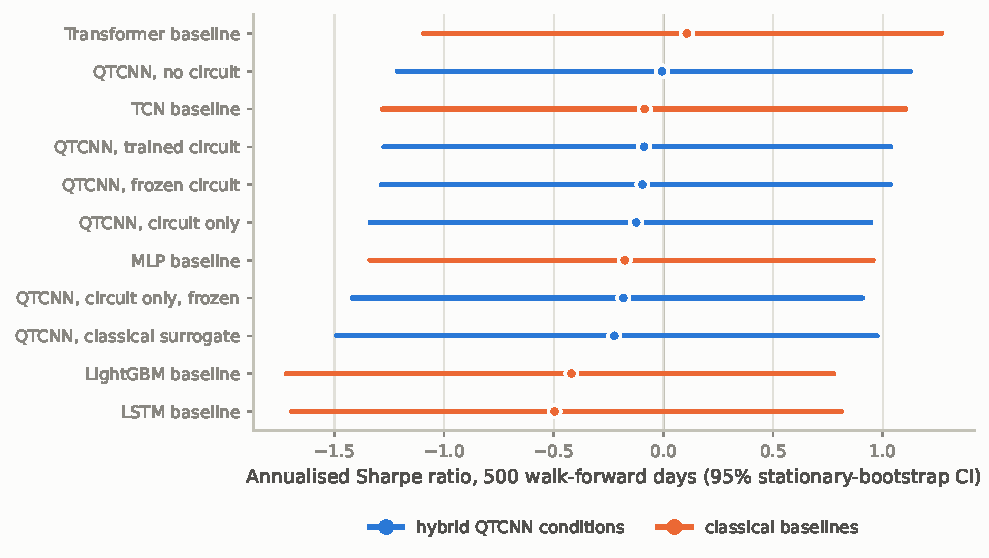
\includegraphics[width=\linewidth]{fig_ablation}
\caption{Annualised Sharpe ratio of each condition on the pooled 500-day
walk-forward track, with 95\% stationary-bootstrap confidence intervals. The
four hybrid conditions differ only in what occupies the quantum position.}
\label{fig:ablation}
\end{figure}

\begin{table}[t]
\centering
\caption{Out-of-sample performance on the pooled walk-forward track (\num{500} trading days, five seeds per condition). Confidence intervals are 95\% stationary bootstrap; DSR is the Deflated Sharpe Ratio deflated by the \num{55} configurations evaluated.}
\label{tab:headline}
\small
\begin{tabular}{lrrrrrr}
\toprule
Condition & Sharpe & 95\% CI & $p$ & DSR & Seed sd & Max DD \\
\midrule
Transformer baseline & +0.107 & [-1.09, +1.27] & 0.85 & 0.17 & 0.31 & -0.128 \\
QTCNN, no circuit & -0.006 & [-1.21, +1.13] & 0.99 & 0.14 & 0.20 & -0.164 \\
TCN baseline & -0.085 & [-1.28, +1.11] & 0.88 & 0.12 & 0.47 & -0.163 \\
QTCNN, trained circuit & -0.088 & [-1.27, +1.04] & 0.87 & 0.11 & 0.14 & -0.176 \\
QTCNN, frozen circuit & -0.096 & [-1.29, +1.03] & 0.86 & 0.11 & 0.15 & -0.178 \\
QTCNN, circuit only & -0.124 & [-1.34, +0.95] & 0.82 & 0.11 & 0.22 & -0.148 \\
MLP baseline & -0.176 & [-1.34, +0.96] & 0.74 & 0.09 & 0.61 & -0.116 \\
QTCNN, circuit only, frozen & -0.183 & [-1.42, +0.91] & 0.74 & 0.09 & 0.26 & -0.159 \\
QTCNN, classical surrogate & -0.224 & [-1.49, +0.97] & 0.71 & 0.08 & 0.35 & -0.192 \\
LightGBM baseline & -0.419 & [-1.72, +0.78] & 0.51 & 0.05 & 0.38 & -0.135 \\
LSTM baseline & -0.496 & [-1.69, +0.81] & 0.44 & 0.04 & 0.13 & -0.233 \\
\bottomrule
\end{tabular}
\end{table}


Nor is any condition distinguishable from the \textsc{None} control, the same
network with the circuit removed. Diebold--Mariano tests on the aligned daily
return series give $p = 0.66$ for \textsc{Trained}, \num{0.66} for
\textsc{Frozen}, \num{0.79} for \textsc{Surrogate} and \num{0.40} for the TCN
baseline; after Romano--Wolf stepdown correction the adjusted $p$ for every hybrid
contrast is \num{0.94}, and the smallest in the family of nine is \num{0.59}
(the circuit-only condition).

The fifth condition bounds the question from the other side. \textsc{QuantumOnly},
whose head sees the circuit output and nothing else, reaches a pooled Sharpe
ratio of \num{-0.251} (95\% CI $[-1.50, +0.85]$, $p = 0.65$) and an information
coefficient of \num{0.0058} ($t = 0.78$), identical to the no-circuit
control's ranking skill to the precision printed (Table~\ref{tab:ic}). It sits
\num{0.26} Sharpe below that control, with a paired standard error of
\num{0.26} ($p = 0.27$; Diebold--Mariano $p = 0.16$, Romano--Wolf $p = 0.56$).
The one-dimensional observable therefore ranks the cross-section as well as
the full hybrid network does, which on this task is barely at all, and placing
the encoder's features beside it recovers the no-circuit level rather than
exceeding it.

The gradient-boosted baseline does not change the picture. LightGBM on the
flattened window reaches a pooled Sharpe ratio of \num{-0.42} (95\% CI
$[-1.72, +0.78]$, $p = 0.51$), an information coefficient of \num{0.0051}
($t = 1.01$) and a turnover of \SI{72}{\percent} per leg per day, the highest
of the ten conditions; early stopping keeps \num{14} trees on average. It sits
\num{0.43} Sharpe below the no-circuit control ($p = 0.20$; Diebold--Mariano
$p = 0.37$). Whatever signal these features carry, the model family that wins
this competition on them extracts no more of it than the networks do.

The sharpest result is Figure~\ref{fig:trained-frozen}, and it is the one
contrast this design can resolve. A non-significant difference is not evidence
of no difference, so we state it as an equivalence rather than as a failure to
reject. On the pooled track the trained circuit and the same circuit frozen at
its initialisation differ by \num{-0.0008} in annualised Sharpe ratio, with a
paired stationary-bootstrap standard error of \num{0.0072}. Two one-sided
tests against a margin of \num{0.03} Sharpe give $p < \num{0.001}$: the
difference is inside that margin, not merely indistinguishable from zero. The
design could have detected a true difference of \num{0.02} at \SI{80}{\percent}
power, so the margin is not an artefact of a blunt instrument. Across the
twenty (fold, seed) cells the two agree to a correlation of \num{1.000}, their
information coefficients never differ by more than $5.5\times10^{-5}$, and their
validation AUCs by more than $3.9\times10^{-5}$.

The contrasts against the no-circuit control are weaker and we report them as
such. Because the study ranks by Sharpe ratio, these are tested twice: by a
Diebold--Mariano statistic on the difference of daily returns, which is a
hypothesis about means, and by a paired bootstrap on the difference of Sharpe
ratios, which is the hypothesis the table is ordered on. The two agree here,
with no contrast significant under either. The trained circuit beats that control by \num{-0.085} Sharpe with a
standard error of \num{0.239}; equivalence holds at a margin of \num{0.50}
($p = \num{0.03}$) but not at \num{0.25} ($p = \num{0.25}$), and the minimum
detectable effect at \SI{80}{\percent} power is \num{0.67}. The honest
statement is therefore that the circuit contributes less than half a Sharpe
unit, not that it contributes nothing. What is established is the narrower and
more diagnostic claim: optimising the circuit's eighteen parameters changes
nothing that freezing them does not change identically, so on this task the
quantum layer acts as a fixed random feature.

This is not simply a failure to train. The circuit does move. Instrumenting the optimiser over a fold, the eighteen
parameters travel an $L_2$ distance of \num{0.044} and \num{0.073} from
initialisations of norm \num{0.416} and \num{0.622}, that is by \SI{11}{\percent}
of their own magnitude. They move, and nothing downstream registers it: the
validation AUC of the trained and frozen conditions differ by at most
$3.9\times10^{-5}$. Whatever the circuit learns, the encoder and head absorb. This is
the behaviour \citet{bermejo2024quantum} predict for a randomly initialised
quantum convolutional network, which they show acts only on low-bodyness
information about its input and is reproduced by a classical surrogate built
from Pauli propagation. Their demonstration is on physics benchmarks; ours is
the same prediction measured on a financial ranking task, and it is
corroborated here by a surrogate that is not merely competitive with the
circuit but statistically equivalent to the network that has no circuit at
all.

Nor is it an artefact of the training budget. Early stopping halts the
walk-forward runs after \num{9.9} epochs on average, so a sceptic could hold
that the circuit was never given time to matter. Re-running both circuit
conditions for the full \num{30} epochs with early stopping disabled moves the
eighteen parameters further, by \SI{26}{\percent} of their initial norm on
average over the twenty cells (range \numrange{3}{70}\,\si{\percent}), and changes
nothing downstream: validation AUC \num{0.5133} for both conditions, differing
by at most $1.4\times10^{-4}$; information coefficients differing by at most
$5.9\times10^{-5}$; per-cell Sharpe ratios correlated at \num{0.999}; a pooled
difference of \num{-0.006} with a paired standard error of \num{0.009}, inside
the \num{0.03} margin ($p = 0.009$, minimum detectable effect \num{0.025}).
The longer budget lowers both conditions equally, from \num{-0.07} to
\num{-0.17} Sharpe, a mild overfitting the pair shares rather than a
contribution of the circuit.

The ordering survives a change of ansatz; the precision does not, and we
report both (Table~\ref{tab:reup}). On the re-uploading circuit with a ring of
entanglers and a global observable (Section~\ref{sec:method:arch}), the
trained and frozen conditions again sit below the no-circuit control, by
\num{0.24} and \num{0.20} Sharpe ($p = 0.45$ and \num{0.58}; Diebold--Mariano
$p = 0.37$ and \num{0.53}), their validation AUCs agree to $1.5\times10^{-4}$, their
per-cell Sharpe ratios correlate at \num{0.998}, and training moves the
\num{48} parameters by \SI{21}{\percent} of their initial norm. Two things
differ from the QCNN. The two conditions are no longer bit-for-bit alike:
information coefficients differ by up to \num{0.011} in a cell, where the QCNN
pair differed by $5.5\times10^{-5}$, so the global observable does let the
parameters reach the score. And the paired standard error of the pooled
Sharpe difference is \num{0.091}, twelve times the QCNN's, so two one-sided
tests certify equivalence only inside a margin of \num{0.25} ($p = 0.005$;
minimum detectable effect \num{0.25}) and not inside \num{0.03}
($p = 0.52$). The difference itself is \num{-0.032}, in the frozen circuit's
favour. What transfers across the two families is therefore the claim that
optimising the circuit does not improve on freezing it; the claim that it
changes nothing at all, to \num{0.03} Sharpe, is established for the QCNN
and bounded at \num{0.25} for the second family.

\begin{table}[t]
  \centering
  \caption{Second ansatz family (data re-uploading, CNOT ring, mean of $Z$
  over all wires) on the Tokyo walk-forward track, \num{500} days, five
  seeds; the no-circuit control is the one of Table~\ref{tab:headline}.
  Bootstrap 95\% intervals and $p$ against zero; information coefficient with
  its Newey--West $t$; $\Delta$ is the pooled Sharpe difference from the row
  above it with its paired standard error; TOST gives the smallest of the
  margins \num{0.03}, \num{0.10}, \num{0.25} at which equivalence holds at
  \SI{5}{\percent}.}
  \label{tab:reup}
  \small
  \begin{tabular}{lrcrrrr}
    \toprule
    Condition & Sharpe & 95\% CI & $p$ & IC ($t$) & $\Delta$ (s.e.) & TOST \\
    \midrule
    No circuit     & $+0.013$ & [$-1.14$, $+1.18$] & 0.99 & 0.0058 (0.88) & -- & -- \\
    Frozen circuit & $-0.190$ & [$-1.48$, $+0.97$] & 0.75 & 0.0084 (1.04) & $-0.203$ (0.389) & -- \\
    Trained circuit& $-0.222$ & [$-1.48$, $+0.95$] & 0.71 & 0.0077 (0.97) & $-0.032$ (0.091) & 0.25 \\
    \bottomrule
  \end{tabular}
\end{table}

\begin{figure}[t]
\centering
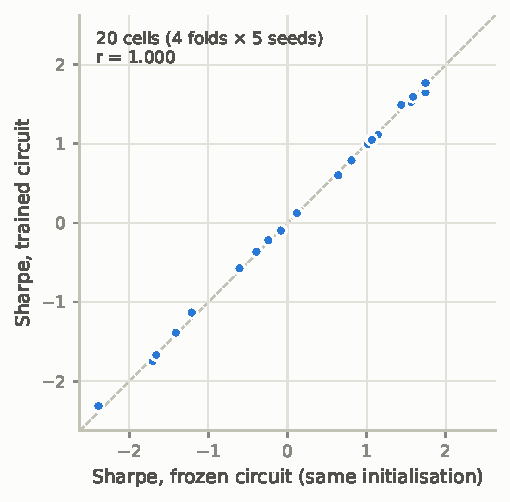
\includegraphics[width=0.55\linewidth]{fig_trained_vs_frozen}
\caption{Per-cell Sharpe ratio, trained circuit against frozen circuit. The
dashed line is the identity.}
\label{fig:trained-frozen}
\end{figure}

\subsection{Ranking skill}
\label{sec:results:ic}

Sharpe ratios are the metric this study is ordered on, but they confound a
model's ranking skill with the portfolio rule applied to it, and the nearest
prior work on the equity cross-section states its headline contrast as a
difference in information coefficient \citep{shen2026quantum}. We therefore
report the ranking statistics directly (Table~\ref{tab:ic}).

\begin{table}[t]
  \centering
  \caption{Ranking skill on both panels: the mean daily information
  coefficient, its Newey--West $t$-statistic, and the Spearman correlation
  between score decile and realised mean forward return as a monotonicity
  measure. Means over the twenty (JPX) and twenty-five (US) cells per condition.}
  \label{tab:ic}
  \small
  \begin{tabular}{lrrrrrr}
    \toprule
    & \multicolumn{3}{c}{JPX} & \multicolumn{3}{c}{US} \\
    \cmidrule(lr){2-4}\cmidrule(lr){5-7}
    Condition & IC & $t_{\mathrm{IC}}$ & Mono. & IC & $t_{\mathrm{IC}}$ & Mono. \\
    \midrule
    QTCNN, trained circuit     & 0.0069 &  0.96 &  0.144 & 0.0020 &  0.08 & -0.369 \\
    QTCNN, frozen circuit      & 0.0070 &  0.96 &  0.144 & 0.0020 &  0.08 & -0.386 \\
    QTCNN, classical surrogate & 0.0066 &  0.87 &  0.177 & 0.0039 &  0.29 & -0.298 \\
    QTCNN, no circuit          & 0.0058 &  0.88 &  0.127 & 0.0029 &  0.25 & -0.324 \\
    QTCNN, circuit only        & 0.0058 &  0.78 &  0.096 &   --   &   --  &   --   \\
    LightGBM baseline          & 0.0051 &  1.01 &  0.032 & 0.0034 &  0.50 & -0.149 \\
    TCN baseline               & 0.0054 &  0.73 &  0.021 & 0.0047 &  0.35 & -0.287 \\
    LSTM baseline              & 0.0058 &  0.75 & -0.042 & 0.0068 &  0.64 & -0.131 \\
    Transformer baseline       & 0.0060 &  0.77 & -0.046 & 0.0097 &  0.94 & -0.038 \\
    MLP baseline               & 0.0048 &  0.78 &  0.094 & 0.0027 &  0.30 & -0.191 \\
    \bottomrule
  \end{tabular}
\end{table}

Three readings, and the first is the one that matters for the ablation. The
trained and frozen circuits agree on every ranking statistic to the precision
printed: identical information coefficients to four decimal places, identical
$t$-statistics, identical monotonicity. The equivalence of
Section~\ref{sec:results:ablation} is therefore not an artefact of the
portfolio rule washing out a difference in the scores; the scores themselves
are the same.

Second, the effect sizes place this study where it belongs in the literature.
The largest difference in information coefficient between any hybrid condition
and the no-circuit control is \num{0.0012} on JPX, against the
\num{0.005} that \citet{shen2026quantum} report as an indistinguishable
kernel-swap contrast on Chinese A-shares, and no $t$-statistic on either panel
reaches \num{1}. Nothing here is a large effect measured imprecisely; the
effects are small.

Third, ranking skill does not translate into realised Sharpe, and on the US
panel it is actively misleading. Every condition has a positive mean
information coefficient there while every condition loses money, and every
decile monotonicity is negative --- the score orders the cross-section in the
direction opposite to realised returns at the extremes, which is where a
long--short book trades. The same dissociation, in the other direction, is what
Section~\ref{sec:results:reeval} finds in the reference implementation, whose
best-performing model has the worst information coefficient of nine. A paper
reporting only one of these two families of statistic can reach either
conclusion it prefers.

\subsection{What does vary}
\label{sec:results:seeds}

Figure~\ref{fig:seeds} shows why single-seed comparisons of these models cannot
be trusted. The seed controls only which \num{60000} of roughly \num{190000}
labelled training sequences a fold draws, yet within a fold the spread across
seeds (standard deviation \numrange{0.12}{1.70} in Sharpe units, and up to
\num{4.39} between the best and worst seed of one condition) exceeds every
between-condition difference in Table~\ref{tab:headline}. Fold 2, which covers
the 2020 recovery, is negative in \num{47} of its \num{50} cells; fold 3 is
positive in almost all of its. On this task the training draw and the test regime
matter, and the architecture does not.

\begin{figure}[t]
\centering
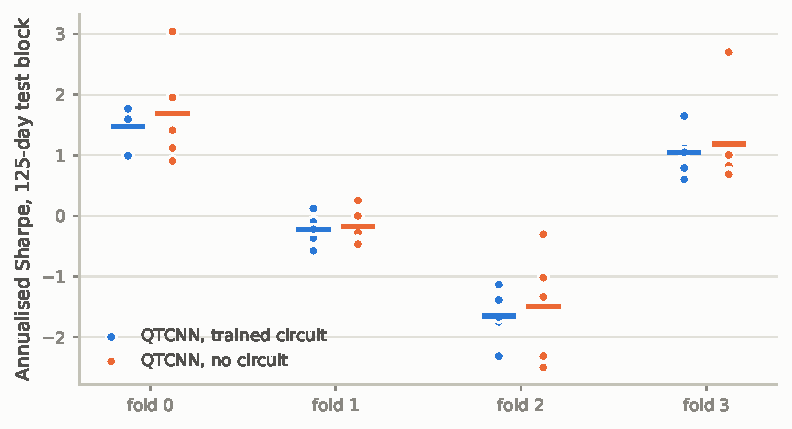
\includegraphics[width=0.9\linewidth]{fig_seed_spread}
\caption{Sharpe ratio per 125-day test block, one point per seed, for the
trained-circuit model and the no-circuit control. Bars mark seed means.}
\label{fig:seeds}
\end{figure}

The combinatorially symmetric cross-validation estimate of the probability of
backtest overfitting across the ten conditions is \num{0.67}: choosing the
in-sample best of them lands below the out-of-sample median in two
partitions out of three, worse than choosing at random.

\subsection{Transaction costs}
\label{sec:results:costs}

Turnover runs from \SI{34}{\percent} (LSTM) to \SI{72}{\percent} (LightGBM) of
each leg per day, and from \SI{49}{\percent} to \SI{54}{\percent} across the
five hybrid conditions. Figure~\ref{fig:cost} charges a round-trip cost on the
traded fraction of both legs. On the pooled track, break-even exists for
exactly one of the ten conditions, the no-circuit control at
\SI{0.06}{bps}, because the other nine have a negative gross mean return
before any cost is charged. Averaging the per-cell break-evens instead, as is
sometimes done, gives a far more flattering \numrange{2.8}{6.5}\,bps, but that
average is taken over only the nine to twelve cells in twenty whose gross
return was positive, and it is not comparable across conditions. At
\SI{5}{bps} the mean per-cell net Sharpe ratio runs from \num{-0.80} to
\num{-2.94}, and at \SI{10}{bps} from \num{-1.65} to \num{-5.63}. The reference implementation's own output, re-scored with the same procedure,
breaks even at \SI{7.4}{bps} on a turnover of \SI{24}{\percent}
(Section~\ref{sec:results:reeval}); neither figure describes a strategy that
could be traded.

\begin{figure}[t]
\centering
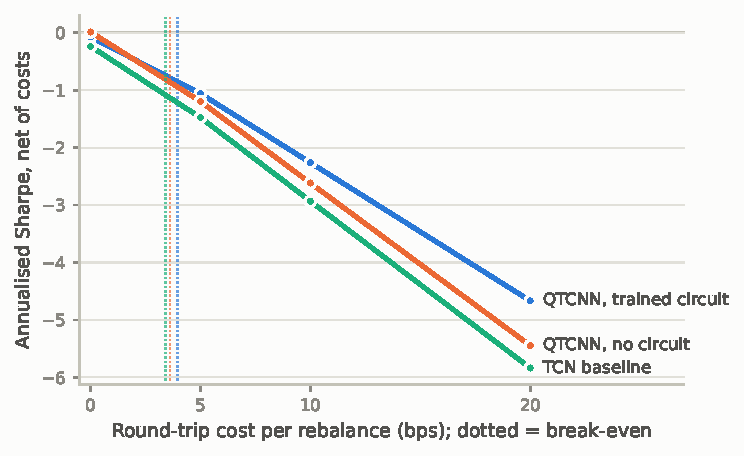
\includegraphics[width=0.75\linewidth]{fig_cost}
\caption{Annualised Sharpe net of round-trip transaction costs. Net Sharpe is
linear in cost at fixed turnover; dotted verticals mark break-even.}
\label{fig:cost}
\end{figure}

\subsection{Is the quantum signal at least orthogonal?}
\label{sec:results:spanning}

A model that loses head-to-head can still earn a place in an ensemble if its
return is not spanned by the alternatives. It is not. Regressing the
trained-circuit model's daily return on the four neural baselines gives
$R^2 = 0.936$ with an annualised intercept of \num{+0.024} and
$t = 1.07$ ($p = 0.28$); regressing it on its own no-circuit twin alone gives
$R^2 = 0.939$ and $t = -0.48$. Pairwise return correlations with the
classical models run from \num{0.89} to \num{0.97}, and an equal-weight blend
with any of them remains negative.

\subsection{A second market}
\label{sec:results:us}

If the null is a property of the task rather than of one exchange, it should
reappear elsewhere. We repeat the entire protocol on the US panel of
Section~\ref{sec:data-us}: the same conditions (nine; the circuit-only
condition was run on Tokyo only), the same code path, the
same five seeds, five walk-forward folds giving \num{625} pooled out-of-sample
days. Table~\ref{tab:headline-us} reports the result.

\begin{table}[t]
\centering
\caption{Out-of-sample performance on the pooled walk-forward track for the US panel (\num{625} trading days, five seeds per condition). Confidence intervals are 95\% stationary bootstrap; DSR is the Deflated Sharpe Ratio deflated by the \num{55} configurations evaluated.}
\label{tab:headline-us}
\small
\begin{tabular}{lrrrrrr}
\toprule
Condition & Sharpe & 95\% CI & $p$ & DSR & Seed sd & Max DD \\
\midrule
LSTM baseline & -0.655 & [-1.83, +0.50] & 0.28 & 0.00 & 0.55 & -0.402 \\
LightGBM baseline & -0.672 & [-2.00, +0.58] & 0.32 & 0.00 & 0.32 & -0.229 \\
Transformer baseline & -1.158 & [-2.34, +0.09] & 0.09 & 0.00 & 0.42 & -0.503 \\
QTCNN, no circuit & -1.441 & [-2.75, -0.05] & 0.05 & 0.00 & 0.16 & -0.532 \\
QTCNN, frozen circuit & -1.463 & [-2.75, -0.09] & 0.05 & 0.00 & 0.23 & -0.535 \\
QTCNN, trained circuit & -1.464 & [-2.74, -0.09] & 0.04 & 0.00 & 0.22 & -0.535 \\
QTCNN, classical surrogate & -1.491 & [-2.79, -0.14] & 0.04 & 0.00 & 0.28 & -0.535 \\
MLP baseline & -1.563 & [-2.92, -0.17] & 0.04 & 0.00 & 0.46 & -0.481 \\
TCN baseline & -2.026 & [-3.38, -0.64] & 0.01 & 0.00 & 0.27 & -0.530 \\
\bottomrule
\end{tabular}
\end{table}


The equivalence replicates, and more tightly than in Tokyo. The trained and
frozen circuits differ by \num{-0.005} Sharpe with a paired standard error of
\num{0.0075}; two one-sided tests against a \num{0.03} margin give
$p = \num{0.0005}$, and the minimum detectable effect at \SI{80}{\percent}
power is \num{0.02}. Their per-cell Sharpe ratios correlate at \num{0.9992}
and their pooled daily returns at \num{0.9999}. Against the no-circuit
control the picture is again weaker: equivalence holds at a \num{0.50} margin
and not at \num{0.25}, with a minimum detectable effect of \num{0.41}. No
Diebold--Mariano contrast is significant, nor is any paired bootstrap test of
the Sharpe difference itself, and nothing survives the Romano--Wolf correction,
whose smallest adjusted $p$ is \num{0.17}, for the LightGBM baseline.

What changes is the sign and, unlike the walk-forward on Tokyo data, the level.
Every condition loses money over this window, which runs from March 2019 to
September 2021 and contains both the COVID crash and the 2021 reversal, and for
three of them --- both circuit conditions and the TCN baseline --- the loss is
itself significant at the \SI{5}{\percent} level. The gross mean return is
negative for all nine, so no condition has a break-even transaction cost at
all. The four hybrid conditions cluster between \num{-1.24}
and \num{-1.44} while the four classical baselines sit between \num{-0.67}
(LightGBM) and \num{-0.85}; the gap is not significant under any test we apply, but it runs
against the hybrid family rather than for it. The backtest-overfitting
probability is \num{0.31}.

We draw one negative lesson from this panel about our own first attempt at it.
The pairwise return correlations across the eight network conditions run from
\num{0.53} to \num{1.000}, not the near-unity we initially measured: that
figure came from a single contaminated security-day, described in
Section~\ref{sec:data-us}, and the inference we had drawn from it --- that the
conditions move as one because they track a single signal --- was an artefact
of the error rather than a finding. The equivalence between trained and frozen
survived the correction unchanged, because a shared bad day cancels in a paired
difference; every level statistic on the panel did not.

Taken with Section~\ref{sec:results:ablation}: in two markets, on different
calendars, with different signs of gross performance, optimising the circuit
changes nothing that freezing it does not change identically, to within a
margin of \num{0.03} Sharpe that the design is powered to resolve.

\subsection{Re-evaluating the reference implementation}
\label{sec:results:reeval}

Contribution~4 is an audit, and an audit that only asserts is worth little. We
therefore re-scored the reference implementation's own saved predictions with
the procedure of Section~\ref{sec:protocol}, over the longest out-of-sample
window its outputs support --- \num{241} trading days rather than the \num{22}
it reported --- leaving its models, features and training untouched.
Table~\ref{tab:reeval} is the result.

\begin{table}[t]
  \centering
  \caption{The reference implementation's nine models, re-scored on
  \num{241} out-of-sample days (2020-12-10 to 2021-12-03) with annualised
  metrics, \SI{95}{\percent} stationary-bootstrap intervals, Deflated Sharpe
  Ratios and Newey--West information-coefficient $t$-statistics. Break-even is
  omitted where the gross return is not positive. Nothing else about the
  pipeline was changed.}
  \label{tab:reeval}
  \small
  \begin{tabular}{lrcrrrrr}
    \toprule
    Model & Sharpe & 95\% CI & $p$ & DSR & IC & $t_{\mathrm{IC}}$ & B/E (bps) \\
    \midrule
    QTCNN (reference)  &  1.80 & [-0.03,  3.79] & 0.07 & 0.54 & 0.0016 &  0.42 & 7.4 \\
    Transformer        &  0.46 & [-0.88,  2.04] & 0.53 & 0.11 & 0.0025 &  0.65 & 2.7 \\
    QLSTM              &  0.13 & [-1.42,  1.75] & 0.85 & 0.06 & 0.0132 &  2.37 & 0.8 \\
    LightGBM ranker    & -0.32 & [-2.34,  1.51] & 0.78 & 0.02 & 0.0060 &  1.52 & --  \\
    QNN                & -0.43 & [-2.31,  1.42] & 0.66 & 0.02 & 0.0148 &  2.10 & --  \\
    MLP                & -0.56 & [-2.24,  1.39] & 0.60 & 0.01 & 0.0134 &  2.57 & --  \\
    LSTM               & -0.59 & [-2.31,  1.27] & 0.49 & 0.01 & 0.0030 &  1.05 & --  \\
    PQC + LightGBM     & -0.76 & [-2.38,  1.06] & 0.39 & 0.01 & 0.0064 &  2.21 & --  \\
    QCNN-LSTM          & -2.15 & [-4.22, -0.17] & 0.04 & 0.00 & 0.0018 &  0.70 & --  \\
    \bottomrule
  \end{tabular}
\end{table}

Three things follow, and none of them requires disagreeing with the reference
implementation about anything except how it was scored.

First, the headline survives the longer window in point estimate but not in
inference. The quantum model is still ranked first, at an annualised Sharpe
ratio of \num{1.80}, but its bootstrap interval spans zero, its $p$-value is
\num{0.07}, and its Deflated Sharpe Ratio is \num{0.54} against the \num{0.95}
a claim requires. Eleven-fold more out-of-sample data does not convert the
result into a significant one; it reveals that the original window was too
short to tell.

Second, and more diagnostically, the ranking by Sharpe ratio and the ranking by
information coefficient are close to opposed. The quantum model has the
\emph{lowest} information coefficient of the nine (\num{0.0016},
$t = \num{0.42}$), while the three models whose information coefficients are
individually significant --- MLP at $t = \num{2.57}$, PQC\,+\,LightGBM at
\num{2.21}, QNN at \num{2.10} --- all have negative Sharpe ratios. A model that
ranks the cross-section better than its rivals and earns less from it is not
being rewarded for its ranking. On a \num{22}-day window that pattern is
invisible; over \num{241} days it is the most informative thing in the table.

Third, costs decide the rest. The reference model turns over \SI{24}{\percent}
of each leg per day and breaks even at \SI{7.4}{bps}; three of the nine have a
break-even at all, and the best of those is under \SI{8}{bps}. None of the nine
describes a strategy that could be traded at institutional costs, which is a
statement about the task and not about any of the architectures in it.

\subsection{Circuit-level diagnostics}
\label{sec:results:diagnostics}

The negative result above is not explained by the circuit being untrainable.
Figure~\ref{fig:barren} plots the variance of a circuit parameter's gradient at
random initialisation from two to twelve qubits: it moves from
$3.1\times10^{-3}$ to $2.0\times10^{-3}$, a fitted log-variance slope of \num{-0.036}
per qubit against the \num{-0.69} an exponential $2^{-n}$ decay would give.
The shared-parameter construction keeps the parameter count at $6L$ regardless
of width, and the measured observable is local, which are the conditions under
which barren plateaus are avoided. Expressibility, measured as KL divergence
from the Haar fidelity distribution, falls from \num{0.188} to \num{0.078}
between one and three layers at eight qubits, so the circuit is neither
degenerate nor flat. It is trainable; training it simply does not help.

\begin{figure}[t]
\centering
\begin{subfigure}[t]{0.48\linewidth}
  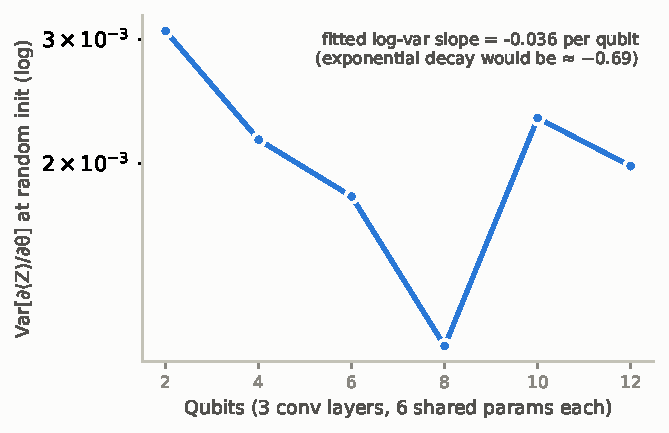
\includegraphics[width=\linewidth]{fig_barren}
  \caption{Gradient variance against register width.}
  \label{fig:barren}
\end{subfigure}\hfill
\begin{subfigure}[t]{0.48\linewidth}
  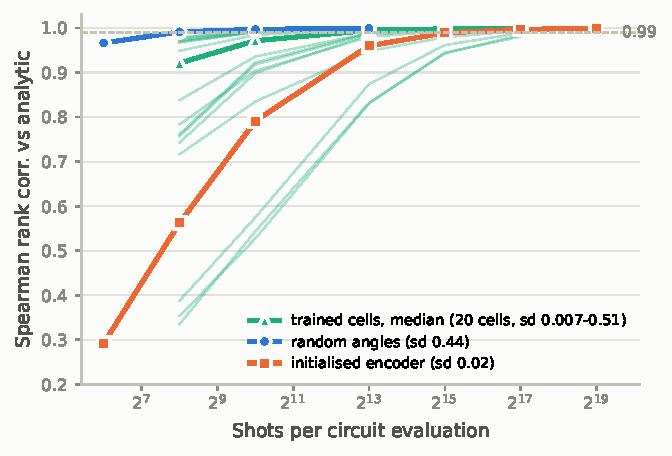
\includegraphics[width=\linewidth]{fig_shots}
  \caption{Rank preservation against shot budget, at both input
  distributions.}
  \label{fig:shots}
\end{subfigure}
\caption{Circuit-level diagnostics at eight qubits and three layers.}
\end{figure}

Figure~\ref{fig:shots} addresses deployment, and it is the one diagnostic in
this section whose answer depends on where the circuit's inputs come from. The
strategy consumes a ranking, so the relevant quantity is the Spearman
correlation between finite-shot and analytic scores within a trading date. On
the uniform random angles a circuit-level scan naturally uses, that correlation
is \num{0.991} at \num{256} shots and \num{0.9996} at \num{8192}, and the
implied budget is undemanding.

Those inputs are not the ones the model produces. Pushing real feature windows
through the encoder and measuring the spread of the circuit output
\emph{within} a cross-section gives a standard deviation of \num{0.018},
against \num{0.443} for random angles --- a factor of \num{24}. Shot
requirements scale with the spread of the quantities being ranked, and at the
real spread the same measurement gives a rank correlation of \num{0.56} at
\num{256} shots, \num{0.79} at \num{1024} and \num{0.96} at \num{8192}. Reaching
\num{0.99} takes about \num{32768} shots per security and reaching \num{0.997}
about \num{131072} (Table~\ref{tab:shots}). Scoring \num{2000} securities daily
therefore costs between $7\times10^{7}$ and $3\times10^{8}$ circuit executions
per trading day, two orders of magnitude above what the random-input scan
implies.

\begin{table}[t]
  \centering
  \caption{Rank preservation against shot budget, measured at two input
  distributions: uniform random angles, and the circuit inputs the encoder
  actually produces on real trading dates (12 dates, 300 securities each,
  within-date Spearman correlation against the analytic score).}
  \label{tab:shots}
  \small
  \begin{tabular}{rrr}
    \toprule
    Shots per security & Random angles (sd \num{0.443}) & Real cross-sections (sd \num{0.018}) \\
    \midrule
    64      & --      & 0.29 \\
    256     & 0.991   & 0.56 \\
    1\,024  & 0.997   & 0.79 \\
    8\,192  & 0.9996  & 0.96 \\
    32\,768 & --      & 0.989 \\
    131\,072& --      & 0.997 \\
    524\,288& --      & 0.9993 \\
    \bottomrule
  \end{tabular}
\end{table}

The mechanism is worth stating because it is a property of the task rather than
of the device. Cross-sectional normalisation and a trained encoder map a day's
securities into a narrow band of embedding angles, so the observable they
produce is concentrated; ranking within that band is a fine discrimination and
finite sampling resolves it slowly. Exponential concentration of quantum
observables is a known obstacle for kernels and reservoirs as system size
grows~\citep{miroszewski2024search}; what this measurement shows is a
task-induced version of it that is already severe at eight qubits, where the
system is far too small for the asymptotic argument to bite. A circuit-level
scan on random inputs cannot see it, which is a reason to measure shot budgets
on the deployed input distribution rather than a convenient one.

Gate noise, by contrast, is invisible at those budgets. Depolarising noise
scales a Pauli expectation by an input-independent factor, so it cannot reorder
scores; the rank correlation is \num{1.0000} at every rate up to $p = 0.05$
whether the rate is uniform across wires or drawn per wire. Under heterogeneous
depolarising noise at \num{1024} shots the correlation is \num{0.997} at
$p = 0$ and \num{0.997} at $p = 0.05$: sampling accounts for all of the
degradation. Amplitude damping, which is non-unital, produces a mean shift in
$\langle Z\rangle$ growing linearly to \num{0.026} at $\gamma = 0.05$ while
depolarising produces none --- confirming the measurement can distinguish the
two --- and still leaves the rank correlation above \num{0.9997}. For this
circuit and observable the deployment constraint is the sampling budget, not
device fidelity.

\subsection{Locked holdout}
\label{sec:results:holdout}

The supplemental window, 2021-12-06 to 2022-06-24 (\num{135} trading days),
was evaluated once per condition after that condition's design was frozen,
with each condition trained on all data to 2021-08-06 under the same validation
and embargo rules. It was opened for the eight network conditions, then for
the LightGBM baseline, and the eight network conditions were then re-run on it
under the released code because the first run could not be reproduced
(Section~\ref{sec:protocol:holdout}). Table~\ref{tab:holdout} reports the
reproducible run; Appendix~\ref{sec:app:rerun} gives the first.

\begin{table}[t]
\centering
\caption{Locked holdout, 135 trading days. Uncorrected
bootstrap $p$ against zero; Romano--Wolf $p$ across the eight contrasts with
the no-circuit control on this window (the two circuit-only
conditions and the second ansatz family were not); DSR deflated by the
\num{55} configurations (eleven models, five seeds) the study evaluated, using the
empirical dispersion of their Sharpe ratios on this window (sd \num{0.92},
expected maximum under the null \num{2.12}); break-even computed on the
pooled track, undefined where the gross return is not positive.}
\label{tab:holdout}
\small
\begin{tabular}{lrrrrrr}
\toprule
Condition & Sharpe & Seed sd & $p$ & $p_{\mathrm{RW}}$ & DSR & Break-even (bps) \\
\midrule
QTCNN, no circuit          & $+1.83$ & 0.84 & 0.07 & --   & 0.42 & 3.7 \\
QTCNN, classical surrogate & $+1.57$ & 1.08 & 0.18 & 0.95 & 0.34 & 5.5 \\
QTCNN, frozen circuit      & $+1.51$ & 1.05 & 0.17 & 0.95 & 0.33 & 4.4 \\
QTCNN, trained circuit     & $+1.49$ & 1.05 & 0.18 & 0.96 & 0.32 & 4.4 \\
TCN baseline               & $+1.37$ & 0.77 & 0.22 & 0.95 & 0.29 & 3.0 \\
Transformer baseline       & $+0.68$ & 0.87 & 0.47 & 0.54 & 0.15 & 2.1 \\
LSTM baseline              & $+0.67$ & 0.79 & 0.48 & 0.91 & 0.15 & 3.8 \\
LightGBM baseline          & $+0.49$ & 0.76 & 0.72 & 0.33 & 0.12 & 0.6 \\
MLP baseline               & $+0.42$ & 0.77 & 0.68 & 0.37 & 0.11 & 1.1 \\
\bottomrule
\end{tabular}
\end{table}

The window replicates the ablation and not the sign. Trained and frozen
circuits differ by \num{0.02}; the no-circuit control is the best of the four
hybrid conditions and the surrogate is no worse than either circuit; every
Diebold--Mariano contrast between a hybrid condition and the no-circuit control
has $p > 0.70$ (the classical baselines are closer, at \num{0.14} for LightGBM
and \num{0.16} for the MLP; one paired Sharpe-difference test, the MLP's,
reaches $p = 0.046$ uncorrected; none survives correction). Gross Sharpe
ratios are higher for all nine conditions than on the walk-forward track, which is a property of the
period, a stretch on which the cross-section rewarded the momentum and
liquidity features every model shares. The ranking of the nine is not stable
across the two windows: the transformer moves from first to sixth and the
no-circuit control from second to first, while the seed standard deviations
(\numrange{0.76}{1.08}) are wider than before because the window is short. What
is stable is the ablation itself (trained beside frozen, the surrogate no
worse than either, and no contrast significant), which is the quantity the
design was built to measure.

No condition is distinguishable from zero by the test on this window either.
For the best, the no-circuit control at \num{+1.83}, the percentile interval
just excludes zero ($[+0.02, +3.94]$) while the null-imposed bootstrap gives
$p = 0.07$, and its Deflated Sharpe Ratio is \num{0.42} against the
\num{0.95} a claim would require: deflated by the \num{55} configurations, the
expected maximum Sharpe under the null on \num{135} days is \num{2.12}, above
every row of the table. At \SI{5}{bps} one condition remains positive, the
surrogate at \num{+0.18}; at \SI{10}{bps} none do.

